\documentclass[20pt,margin=1in,innermargin=-4.5in,blockverticalspace=-0.25in]{tikzposter}
\geometry{paperwidth=42in,paperheight=30in}
\usepackage[utf8]{inputenc}
\usepackage{amsmath}
\usepackage{amsfonts}
\usepackage{amsthm}
\usepackage{amssymb}
\usepackage{mathrsfs}
\usepackage{graphicx}
\usepackage{adjustbox}
\usepackage{enumitem}
\usepackage[backend=biber,style=apa]{biblatex}
\usepackage{emory-theme}
\usepackage{caption}
\usepackage{mwe} % for placeholder images


\addbibresource{refs.bib}
\nocite{*}

% set theme parameters
\tikzposterlatexaffectionproofoff
\usetheme{EmoryTheme}
\usecolorstyle{EmoryStyle}

\title{\uppercase{Tree-Based Multiple Imputation Methods}}
\author{Michael Dellermann, Anatol Sluchych, and Jonah Wermter}
\titlegraphic{
\includegraphics[scale=1.3]{fu_logo.jpg}}

% begin document
\begin{document}
\maketitle
\centering
\begin{columns}
    \column{0.32}
    
    \block{1. Motivation}{
        \vspace{-1em}
        \begin{itemize}
            \item Parametric MICE methods: conditional models to be specified for \textit{all} variables with missing data (van Buuren \& Groothuis-Oudshoorn, 2011)
            \vspace{-0.5em}
            \item Still may fail to capture interactive and nonlinear relations among variables as well as non-standard distributions
            \vspace{-0.5em}
            \item Tree-based methods \textit{automatically} capture interactions, nonlinear relations, and complex distributions with no parametric assumptions or data transformations needed (Burgette \& Reiter, 2010)
            \vspace{-0.5em}
            \item Implementation in R: \textit{mice}, \textit{miceRanger}, and \textit{missRanger} packages
        \end{itemize}
    }
    
    \block{2. Tree-based methods}{
        \vspace{-1em}
        Classification and regression trees (CART):
        \vspace{-0.5em}
        \begin{itemize}
            \item seek to approximate  conditional distribution of univariate outcome from multiple predictors
            \vspace{-0.5em}
            \item segment predictor space into non-overlapping regions with relatively homogeneous outcomes
            \vspace{-0.5em}
            \item segments found by recursive binary splits of  predictors
            \vspace{-0.5em}
            \item prediction for observations that fall into the same region is mean (or mode) of response values for training observations in region
            \vspace{-0.5em}
            \item may be very non-robust and have relatively low predictive accuracy 
        \end{itemize}
        
        \vspace{-1.5em}

        \begin{center}
            \captionof{figure}{Example of tree structure. Source: Hastie, Tibshirani, \& Friedman (2009)}
            \begin{tikzfigure}[]
                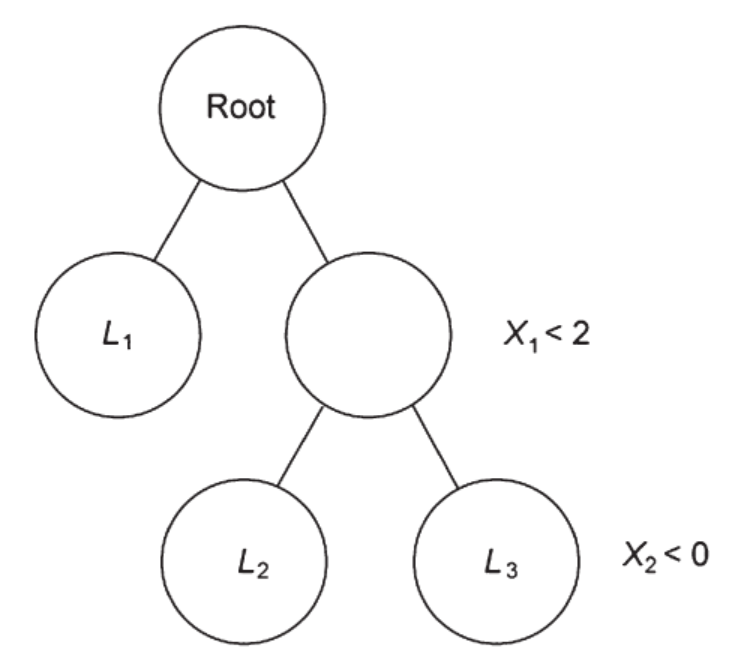
\includegraphics[scale=1.9]{tree.png}
             \end{tikzfigure}
        \end{center}

        \vspace{-3em}
        
        Random forest:
        \vspace{-0.5em}
        \begin{itemize}
            \item \textit{ensemble} method that addresses non-robustness and low predictive accuracy
            \vspace{-0.5em}
            \item average predictions from $B$ non-pruned trees constructed using $B$ bootstrapped training sets 
            \vspace{-0.5em}
            \item \textit{decorrelates} trees by performing each split on \textit{randomly} chosen subset of predictors
            \vspace{-0.5em}
            \item accurate model to impute missing values (Stekhoven \& Bühlmann, 2012)
            \vspace{-1em}
        \end{itemize} 
    }

    \block{3. Imputation algorithm}{
    \vspace{-1em}

  %      \begin{itemize}
  %          \item sequential CART imputation algorithm
  %          \item  order the variables from least amount to largest amount of missing data
  %          \item minimum leaf size of 5 and the splitting criteria of a deviance greater than 0.0001
  %          \item trees are not pruned to minimize bias
  %          \item size of trees modulated by requiring a minimum number of observations in each leaf and by %controlling the minimum heterogeneity in the values in the leaf in order to consider it for further splitting     
  %          \item We take draws from the predictive distribution by sampling elements from the leaf that corresponds to the covariate values of the record of interest
  %          \item  actually perform a Bayesian bootstrap within each leaf before sampling.
  %     \end{itemize}

    
    4-steps algorithm:
    \vspace{-0.5em}
    \begin{enumerate}
        \item Initial values for missing values filled in as follows:
        \vspace{-0.5em}
        \begin{enumerate}
            \item Define matrix $Z$ equal to $Y_c$ (ordered matrix according to missingness)
            \vspace{-0.25em}
            \item Impute missing values in $Y_i$, $i=1, ... p_1$, using tree-based method on $Z$ and append completed version of $Y_i$ to $Z$ prior to incrementing $i$             
        \end{enumerate}
    \vspace{-1em}
    \item  Replace originally missing values of $Y_i$, $i=1, ... p_1$, with tree-based methods on $Y_{-i}$
    \vspace{-0.5em}
    \item Repeat step 2 $l$  times ($l$  iterations)
    \vspace{-0.5em}          
    \item Repeat steps 1–3 $m$ times and obtain $m$ imputed sets
    \vspace{-0.5em}
    \item Pool $m$ datasets to one completed according to Rubin’s rules  
    \end{enumerate}  
    
    \vspace{-1em}
}

    \column{0.36}
        \block{4. Comparison \textit{mice}, \textit{miceRanger} \& \textit{missRanger}}{
        \vspace{-2em}
        \begin{itemize}
            \item Packages \textit{mice} and \textit{miceRanger} implement van Buuren’s multivariate imputation by chained equations, \textit{missRanger} by default single imputations (based on \textit{missForest})
            \vspace{-0.5em}
            \item \textit{mice} supports variety of imputation methods, \textit{miceRanger} \& \textit{missRanger} only random forest
            \vspace{-0.5em}
            \item All by default use \textit{ranger} package for random forests (van Buuren, 2023; Mayer, 2023; Wilson, 2022), which claims to be faster and more efficient with larger data sets and complex settings than common R packages (Wilson, 2022)
            \vspace{-0.5em}
            \begin{itemize}
                \item[$\Rightarrow$] core functions written in C++ (faster than R, compiled vs. interpreted code) (Wright \& Ziegler, 2017)
                \vspace{-0.5em}
            \end{itemize}
            \item main differences in default values and variety of analytical functions
        \end{itemize}
        
        \vspace{-1em}
    }
    
        \block{5. Empirical simulation study}{ 
        \vspace{-1em}
        Empirical data set:
        \vspace{-0.5em}
        \begin{itemize}
            \item RAND's Health Insurance Experiment:  $n = 20185$, $k = 46$
        \end{itemize}
        
        \vspace{-0.5em}
        
        Missing data mechanisms:
        \vspace{-0.5em}
        \begin{itemize}
            \item p=25\% and 50\%
        \end{itemize}
        \vspace{-1.5em}
        \begin{itemize}
            \item MAR: $P(mdvis\_miss \mid xage<25) = p$,  $P(mdvis\_miss \mid mhi>74) = p$ 
            \vspace{-0.5em}
            \item MCAR: $P(income\_miss) = p$, $P(educdec\_miss) = p$
        \end{itemize}
        
        \vspace{-0.5em}
        
        Monte Carlo simulation: $R$ = 100, $M$ = 5, $n$ = 1000, $niter$ = 10, $nrtree$ = 10
        \vspace{-0.5em}
        \begin{itemize}
            \item six subsets: three focus on data types, three on dataset size
        \end{itemize}
        \vspace{-1em}
    }


        \block{6. Results}{
        
        \vspace{-1em}

        \begin{center}
            \captionof{table}{Simulation results}
            \vspace{-0.5em}
            \begin{tabular}{|l|l|rrr|}
             \hline   
             Metric &  Method & Bias \hspace{10mm} & MSE \hspace{5mm} & Coverage\\
             \hline
             mean(income) & BD & 1.98  & 15,186 & 0.96\\
             mean(income) & CC & 7.39  & 26,003 & 0.96\\
             mean(income) & mice-CART & 12.44 & 23,660 & 0.94\\
             mean(income) & mice-RF & 8.48 & 23,922 & 0.94\\
             mean(income) & miceRanger & -1.33 & 22,833 & 0.92\\
             mean(income) & missRanger  & 20.02 & 23,362 & 0.86 \\
             \hline
             mean(mdvis|xage>25) & BD & 0.01 & 0.05 & 0.95\\
             mean(mdvis|xage>25) & CC & 0.01 & 0.05 & 0.95\\
             mean(mdvis|xage>25) & mice-CART & 0.01 & 0.05 & 1\\
             mean(mdvis|xage>25) & mice-RF & 0.01 & 0.05 & 1\\
             mean(mdvis|xage>25) & miceRanger & 0.01 & 0.05 & 0.95\\
             mean(mdvis|xage>25) & missRanger  & 0.01 & 0.05 & 0.95\\
             \hline
             reg. intercept (ghindx) & BD & 0.10 & 4.03 & 0.95\\
             reg. intercept (ghindx) & CC & -1.72 & 28.69 & 0.93\\
             reg. intercept (ghindx) & mice-CART & 0.54 & 6.43 & 0.94\\
             reg. intercept (ghindx) & mice-RF & 0.78 & 6.03 & 0.95\\
             reg. intercept (ghindx) & miceRanger & -1.30 & 9.55 & 0.89\\
             reg. intercept (ghindx) & missRanger  & -3.36 & 23.24 & 0.69\\
             \hline
        \end{tabular}
        \end{center}
    }

    \column{0.32}   

        \block{}{
        \vspace{-2.5em}

        \begin{center}
            \captionof{figure}{Imputation time per method for levels of missingness}
            \vspace{-1em}
            \begin{tikzfigure}[]
                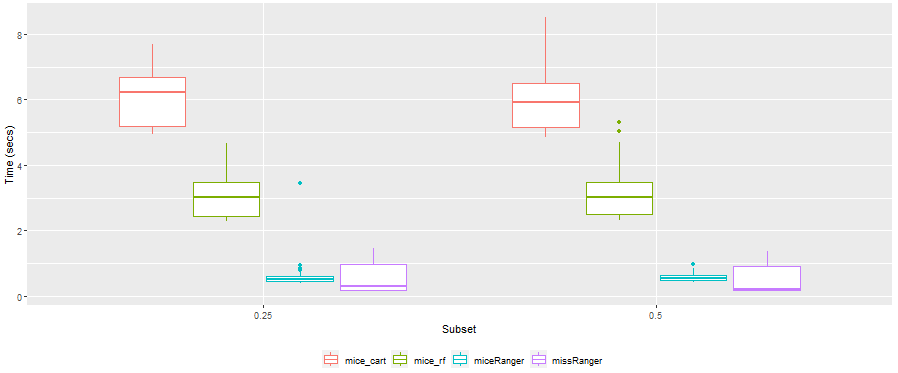
\includegraphics[width=1\linewidth]{plot_comp_time_mis.png}
            \end{tikzfigure}
        \end{center} 
        \vspace{-2em}
        
        \begin{center}
            \captionof{figure}{Imputation time per subset per method}
            \vspace{-0.5em}
            \begin{tikzfigure}[]
                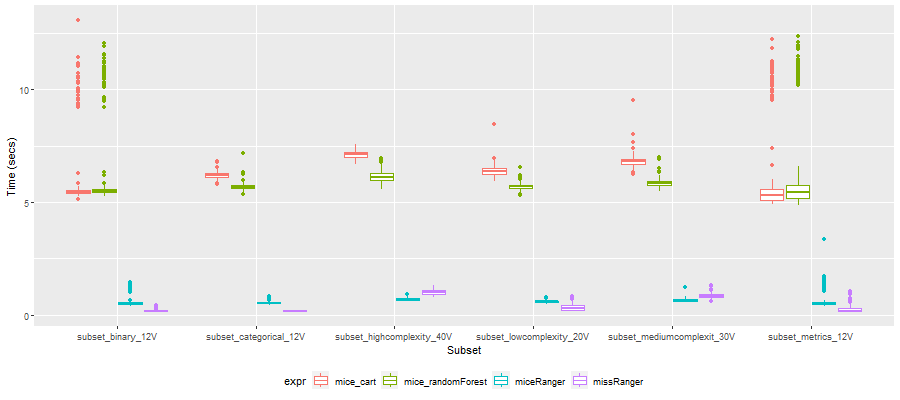
\includegraphics[width=1\linewidth]{plot_comp_time.png}
            \end{tikzfigure}
        \end{center}
        \vspace{-2em}

        \begin{center}
            \captionof{figure}{Imputation time vs m}
            \vspace{-0.5em}
            \begin{tikzfigure}[]
                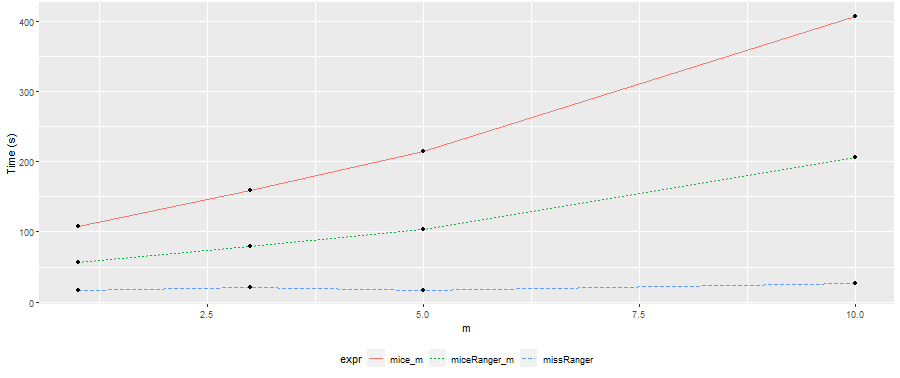
\includegraphics[width=1\linewidth]{plot_computational_time_vs_m.png}
            \end{tikzfigure}
        \end{center}
        \vspace{-2em}

        % \begin{center}
        %    \captionof{figure}{Coverage rate by model}
        %    \vspace{-0.5em}
        %    \begin{tikzfigure}[]
        %        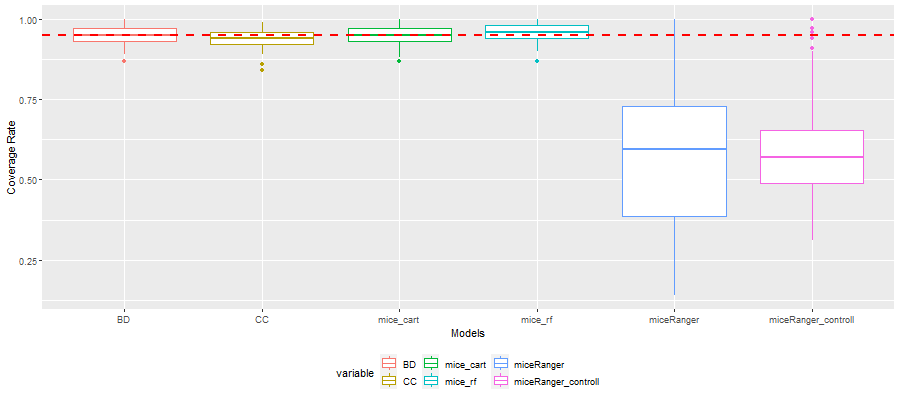
\includegraphics[width=1\linewidth]{plot_coverage.png}
        %    \end{tikzfigure}
        % \end{center} 
        % \vspace{-1em}

    }
  
    \block{7. Conclusion}{
    
    \vspace{-2em}
    
    \begin{itemize}
        \item Speed \& robustness: \textit{miceRanger} \& \textit{missRanger} are $\sim$11x faster than \textit{mice} using standard R implementations and $\sim$6x faster than \textit{mice} using \textit{ranger}.
        \vspace{-0.5em}
        \item Scalability: \textit{missRanger} scales best with increased number of observations, imputations and trees, \textit{miceRanger} performing similarly
        \vspace{-0.5em}
        \item  Efficiency: Despite faster speed of \textit{miceRanger} and \textit{missRanger}, \textit{mice} demonstrates superior imputation accuracy
        \vspace{-0.5em}
        \item User-friendliness: \textit{mice} facilitates post-imputation analysis; \textit{miceRanger} demands manual data handling
        \vspace{-0.5em}
        \item Practical recommendation: Choose \textit{miceRanger} for speed, \textit{mice} for in-depth research analysis
    \end{itemize}
    
    \vspace{-1em}
    }
    
    \block{References}{
        \vspace{-2em}
        \begin{footnotesize}
        \printbibliography[heading=none]
        \end{footnotesize}
    }
\end{columns}
\end{document}

        \centering
        \begin{tabular}{|l|l|lll|}
             \hline   
             Metric &  Method & Bias \hspace{3mm} & MSE \hspace{3mm} & Coverage \hspace{3mm}\\
             \hline
             mean(age) & BD & NA & NA & NA\\
             mean(age) & CC & NA & NA & NA\\
             mean(age) & CART & NA & NA & NA\\
             mean(age) & RandomForest & NA & NA & NA\\
             mean(age) & miceRanger  & NA & NA & NA \\
             \hline
             mean(educ) & BD & NA & NA & NA\\
             mean(educ) & CC & NA & NA & NA\\
             mean(educ) & CART & NA & NA & NA\\
             mean(educ) & RandomForest & NA & NA & NA\\
             mean(educ) & miceRanger  & NA & NA & NA \\
             \hline
             $\rho$(mdvis, hltg)  & BD & NA & NA & NA\\
             $\rho$(mdvis, hltg) & CC & NA & NA & NA\\
             $\rho$(mdvis, hltg) & CART & NA & NA & NA\\
             $\rho$(mdvis, hltg) & RandomForest & NA & NA & NA\\
             $\rho$(mdvis, hltg) & miceRanger  & NA & NA & NA \\
             \hline
             reg.(mhi)  & BD & NA & NA & NA\\
             reg.(mhi) & CC & NA & NA & NA\\
             reg.(mhi) & CART & NA & NA & NA\\
             reg.(mhi) & RandomForest & NA & NA & NA\\
             reg.(mhi) & miceRanger  & NA & NA & NA \\
             \hline
        \end{tabular}
        \captionof{table}{Simulation results}
}



    
        Following Burgette \& Reiter (2009), let $Y$ be $n \times p$ the data matrix arranged as $Y= (Y_p, Y_c)$, where
        \begin{itemize}
            \item $Y_p$ consists of $p_1$ \textit{partially observed} columns, such that moving from left to right, the number of missing elements in each column is nondecreasing
            \item  $Y_c$ remaining completely observed columns
            \item  $Y_{obs}$ set of observed and $Y_{mis}$ set of missing elements 
        \end{itemize}